%%==================================================================%%
%% Author : Tejedo Gonz�lez, Daniel                                 %%
%%          S�nchez Barreiro, Pablo                                 %%
%% Version: 1.0, 10/12/2012                                         %%                   %%                                                                  %%
%% Memoria del Proyecto Fin de Carrera                              %%
%% semantica, interfaz                                       %%
%%==================================================================%%

EMF y EMFText proporcionan una interfaz por defecto para la creaci�n de editores y su posterior uso. Se incluyen algunos aspectos como coloreado de palabras clave y detecci�n instant�nea de errores de sintaxis. Es por eso que ya cont�bamos con gran parte del trabajo hecho, y esta ha sido una de las razones por las que EMFText pareci� m�s conveniente en su momento.

La interfaz del editor desarrollado es parte de la herramienta Eclipse y no puede ejecutarse fuera de su entorno. No tendr�a sentido hacerlo de otro modo, ya que no solo necesitamos las diversas funciones que EMF y EMFText nos proporcionan, sino que la propia herramienta Hydra es tambi�n un plug-in de Eclipse. La figura \ref{figeditor} muestra la interfaz del editor en funcionamiento.

\begin{figure}[t]
\includegraphics[scale=0.34]{semantica/editor.eps}
\caption{Captura de pantalla del editor en funcionamiento}
\label{figeditor}
\end{figure} 

Las caracter�sticas del editor creado por defecto por EMF no son suficientes para satisfacer toda la funcionalidad que debe llevar a cabo, por lo que ha sido necesaria una ligera modificaci�n para poder cumplir con los objetivos de nuestra aplicaci�n. Para poder implementar la sem�ntica es necesario que nuestro editor cargue previamente dos modelos: el modelo de caracter�sticas (lo cual ya ha sido implementado) y una configuraci�n de ese modelo, que es sobre el que se validar�n las restricciones que definamos.

Para permitir que se pueda cargar esa configuraci�n hemos a�adido un bot�n llamado "Validate" que abre una ventana de carga en la que se pide al usuario escoger un fichero de extensi�n .xmi exclusivamente. Una vez cargado, el manejador del bot�n ejecutar� la validaci�n y mostrar� el resultado de la misma en un cuadro de di�logo. Pero esto es tarea de la sem�ntica y ser� explicado en el apartado siguiente. 

\begin{figure}[t]
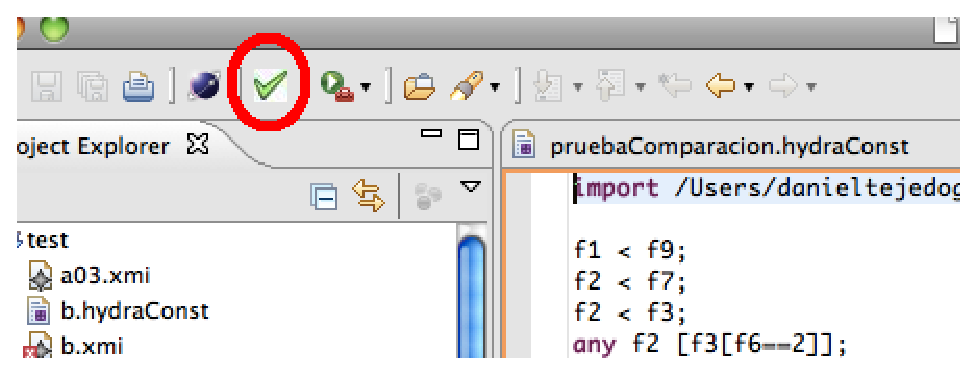
\includegraphics[scale=0.74]{semantica/boton.eps}
\caption{Bot�n que ejecutar� la validaci�n de las restricciones}
\label{figboton}
\end{figure} 

Dado que nuestra aplicaci�n no es sino un plug-in de Eclipse, a�adir el bot�n ha requerido informarse de la Arquitectura de Plug-ins de Eclipse. Sin entrar en demasiados detalles, el proceso consiste en a�adir lo que se conoce como "punto de extensi�n" al plug-in previo. Un punto de extensi�n sirve para dotar a un plug-in de la funcionalidad de otros plug-ins e incorporarla a ellos. En este caso nuestro punto de extensi�n corresponde a uno proporcionado por la propia arquitectura, cuya utilidad es precisamente la de a�adir botones al men� de herramientas de nuestra aplicaci�n.
